\documentclass[]{article}
\usepackage[utf8]{inputenc}
\usepackage{comment}
\usepackage{mathtools}

% For diagrams
\usepackage{tikz}
\usetikzlibrary{automata, positioning, arrows}
\tikzset{
    ->, % makes the edges directed
    >=stealth, % makes the arrow heads bold
    node distance=3cm, % specifies the minimum distance between two nodes. Change if necessary.
    every state/.style={thick, fill=gray!10}, % sets the properties for each ’state’ node
    initial text=$ $, % sets the text that appears on the start arrow
}

\title{Appunti SFB 2023/2024}
\author{Umberto Loria}
\date{Ottobre 2023}

\begin{document}

\begin{titlepage}
\maketitle
\end{titlepage}

\tableofcontents{}
\newpage
\section{Linguaggi formali}

Un \textit{alfabeto} \mbox{$\Sigma$} è un insieme \underline{finito} di elementi (lettere, simboli o caratteri).
\\
Sia \mbox{$\Sigma=\{\sigma_0 ... \sigma_k\}$} alfabeto di \begin{math}k\end{math} simboli con cardinalità \mbox{$|\Sigma|=k$}.
\\
\\
Esempi:

\mbox{$\Sigma=\{a, b, ..., z\}$} alfabeto delle lettere romane minuscole

\mbox{$\Sigma=\{0, 1, ..., 9\}$} alfabeto delle cifre arabe

\mbox{$\Sigma=\{0, 1\}$} alfabeto binario
\\
\\
Una \textit{parola} (o stringa) su un alfabeto è una sequenza (finita) di simboli dell'alfabeto.
Esempio: \mbox{$\Sigma = \{a, c, s\}, w = casa$} parola su \mbox{$\Sigma$}
\\
\\
Un \textit{linguaggio} formale è un insieme di parole su un alfabeto.
\\
Esempio:

Insieme di tutti i programmi sintatticamente validi scritti in C++

Insieme di nomi di variabili in Java
\\
\\
La \textit{cardinalità di un linguaggio} finito è il numero di parole che esso contiene.
Esempi:

\mbox{$L_1=\{a, b, ab\}, |L_1|=3$}

\mbox{$L_2=\{aba, abb\}, |L_2|=2$}
\\
\\
Un linguaggio è \textit{finito} se contiene un numero finito di parole.
\\
Un linguaggio è \textit{non finito} se contiene un numero infinito di parole.


\subsection{Parole}

La \textit{lunghezza} di una parola \mbox{$w$} è definita con \mbox{$|w|$}.
Esempio: \mbox{$|ab| = 2$}.
\\
\\
La parola vuota si indica con \mbox{$\epsilon$}. Essa è l'elemento neutro dell'insieme delle parole ed è l'unica
parola con lunghezza pari a \mbox{$0$}. Quindi vale \mbox{$|\epsilon|=0$}.
\\
\\
Il \textit{numero di occorrenze} del simbolo \mbox{$\sigma$} in una parola \mbox{$w$} è definito con \mbox{$|w|_\sigma$}. Esempio: \mbox{$|aab|_a=2$}.


\subsection{Uguaglianza tra parole}

Sia
\begin{math}
a = a_1...a_k
\end{math}
e
\begin{math}
b = b_1...b_h
\end{math}
con
\begin{math}
k, h \in \mathbf{N},
a_1, ..., a_k, b_1, ..., b_h \in \Sigma
\end{math}.
\\
Allora:
\\
\begin{math}
a=b
\overset{\text{def}}{\Leftrightarrow}
\begin{cases}
k = h \\
\forall i \in \{1, ..., k\} : a_i=b_i
\end{cases}
\end{math}

\newpage
\subsection{Concatenazione di parole}

Sia
\begin{math}
a = a_1...a_k
\end{math}
e
\begin{math}
b = b_1...b_h
\end{math}
con
\begin{math}
k, h \in \mathbf{N},
a_1, ..., a_k, b_1, ..., b_h \in \Sigma
\end{math}.
\\
Allora:
\\
\begin{math}
ab = a_1...a_kb_1...b_h
\end{math}
\\
Questa operazione si chiama concatelazione (o giustapposizione) di parole.
\\
\\
Si noti che \mbox{$\epsilon w = w \epsilon = w$} e che \mbox{$\epsilon \epsilon = \epsilon$}.
\\
\\
L'operazione di concatenazione non gode della proprietà commutativa, infatti con \mbox{$a=anna, b=maria$} si ha
che \mbox{$ab = annamaria \neq mariaanna = ba$}.


\subsubsection{Proprietà associativa della concatenazione}

L'operazione di concatenazione gode invece della proprietà associativa.
Siano \mbox{$a=a_1...a_m, b=b_1...b_n, c=c_1...c_l$} con
\mbox{$a_1, ..., a_m, b_1, ..., b_n, c_1, ..., c_l \in \Sigma, m, n, l \in \mathbf{N}$}
\\
Vale che:
\\
\mbox{$(ab)c = (a_1...a_mb_1...b_n)c_1...c_l = a_1...a_mb_1...b_nc_1...c_l = a_1...a_m(b_1...b_nc_1...c_l) = a(bc)$}


\subsubsection{Stabilità della lunghezza di parole rispetto alla concatenazione}

Siano \mbox{$a=a_1...a_m, b=b_1...b_n$} con
\mbox{$a_1, ..., a_m, b_1, ..., b_n \in \Sigma, m, n \in \mathbf{N}$}
\\
Vale che:
\\
\mbox{$|ab| = |a| + |b| = m + n$}
\\
\\
Dimostrazione diretta:
\\
\mbox{$|ab| = |a_1...a_mb_1...b_n| = |a_1...a_m| + |b_1...b_n| = m + n = |a| + |b|$}
\\
\\
Dimostrazione induttiva:
\\
Passo base:

\mbox{$|ab|=|a_1...a_mb_1...b_n|$}.
\\
Passo induttivo:

Sia
\mbox{$|wv|=|w|+|v|$}
con
\mbox{$w, v \in \Sigma^*, a, b \in \Sigma$}

allora

\mbox{$|wavb| = |wvab| = |wv| + 2 = |w| + |v| + 2 = |w| + |a| + |v| + |b| = |wa| + |vb|$}


\subsection{Prefissi, suffissi e sottostringhe}

Sia \mbox{$x = uyv$} con \mbox{$u, y, z \in \Sigma^*$}, si dicono:

\mbox{$u$} prefisso di \mbox{$x$}

\mbox{$y$} sottostringa di \mbox{$x$}

\mbox{$v$} suffisso di \mbox{$x$}
\\
Una \textit{sottostringa} può essere chiamata anche fattore.
\\
Si noti che vangolo anche le seguenti.

\mbox{$x$} prefisso di \mbox{$x$}

\mbox{$x$} sottostringa di \mbox{$x$}

\mbox{$x$} suffisso di \mbox{$x$}


\subsubsection{Prefissi propri, suffissi propri e sottostringhe proprie}

Siano \mbox{$w, x \in \Sigma^*$}
\\
allora:
\\
\\
\begin{math}
w \text{ prefisso proprio di } x
\overset{\text{def}}{\Leftrightarrow}
\begin{cases}
w \text{ prefisso di } x \\
w \neq x
\end{cases}
\end{math}
\\
\\
\\
\begin{math}
w \text{ sottostringa propria di } x
\overset{\text{def}}{\Leftrightarrow}
\begin{cases}
w \text{ sottostringa di } x \\
w \neq x
\end{cases}
\end{math}
\\
\\
\\
\begin{math}
w \text{ suffisso proprio di } x
\overset{\text{def}}{\Leftrightarrow}
\begin{cases}
w \text{ suffisso di } x \\
w \neq x
\end{cases}
\end{math}



\subsection{Ripetizioni di parola}

Siano \mbox{$ w \in \Sigma^*, m \in \mathbf{N_0} $}:
\\
\mbox{$ w^m = w ... w \text{ m volte} = \Pi_1^m w $}
\\
\\
Definizione ricorsiva:
\\
Passo base: \mbox{$ w^0 = \epsilon $}
\\
Passo ricorsivo: \mbox{$ w^m = w^{m-1} w, \forall m \in \mathbf{N} $}



\subsection{Inversa di una parola}

Sia \mbox{$w = w_1...w_k$} con \mbox{$k \in \mathbf{N}$}.
\\
La parola inversa è \mbox{$w^R = w_k...w_1$}
\\
\\
Definizione ricorsiva:
\\
Passo base: \mbox{$\epsilon^R = \epsilon$}
\\
Passo ricorsivo: Sia \mbox{$w = x \sigma$} con \mbox{$x \in \Sigma^*, \sigma \in \Sigma$}
\\
\mbox{$w^R = (x \sigma)^R = \sigma w^R$}
\\
\\
La inversione di una parola è talvolta chiamata \textit{riflessione}.
\\
\\
Si noti che:
\\
\mbox{$ (x^R)^R = x $}
\\
Dimostrazione:
\\
\mbox{$ (x^R)^R = ((x_1...x_k)^R)^R = (x_k...x_1)^R = x_1...x_k = x $}
\\
\\
Si noti che:
\\
\mbox{$ (xy)^R = y^R x^R $}
\\
Dimostrazione:
\\
\mbox{$ (xy)^R = (x_1...x_k y_1...y_h)^R = y_h...y_1 x_k...x_1 $}



\subsection{Precedenze delle operazioni}

L'elevamento a potenza di una parola ha precedenza rispetto alla concatenazione.
\\
\mbox{$ (ab)^2 = abab \neq abb = ab^2 $}
\\
L'inversione di una parola ha precedenza rispetto alla concatenazione.
\\
\mbox{$ (ab)^R = ba \neq ab = ab^R $}


\subsection{Operazioni unari sui linguaggi}


\subsubsection{Riflessione di un linguaggio}

Sia \mbox{$ L $} un linguaggio su alfabeto \mbox{$ \Sigma $}.
\\
\\
\mbox{$ L^R = \{ w^R | w \in L \} $}
\\
\\
Esempio:
\\
\mbox{$ L_1 = \{ aa, aaa \} = L_1^R $}
\\
\mbox{$ L_2 = \{ aab, aba \} \neq \{ baa, aba \} L_2^R $}
\\
\mbox{$ L_3 = \{ w | |w|_a = |w|_b \} = L_3^R $}



\subsubsection{Prefissi propri di un linguaggio}

Sia \mbox{$ L $} un linguaggio su alfabeto \mbox{$ \Sigma $}.
\\
\\
\mbox{$ Prefissi(L) = \{ w | w = xz \land x \in L \land z \neq \epsilon \} $}

\mbox{$ = \{ w | w \text{ prefisso proprio di una parola in } L \} $}
\\
\\
\mbox{$ L \text{ prefisso } \overset{\text{def}}{\Leftrightarrow}
L \cap Prefissi(L) = \emptyset $}
\\
\\
Oppure, in modo alternativo:
\\
\mbox{$ L \text{ prefisso } \overset{\text{def}}{\Leftrightarrow}
L / Prefissi(L) = L $}
\\
\\
Esempio:
\\
\mbox{$ L_1 \text{ non prefisso } \colon Prefissi(L_1) = \{ \epsilon, a, aa \} $}
\\
\mbox{$ L_2 \text{ prefisso } \colon Prefissi(L_2) = \{ \epsilon, a, aa, ab \} $}
\\
\mbox{$ L_3 \text{ non prefisso } \colon Prefissi(L_3) = \{ \epsilon, a, aa, ab \} $}


\newpage
\subsubsection{Dimostrazione \mbox{$ a^nb^n $} linguaggio prefisso}

\mbox{$ L = \{ a^nb^n | n \in \mathbf{N} \} $}
\\
\begin{math}
L \cap Prefissi(L) = \emptyset
\Leftrightarrow
\begin{cases}
w \in L \Rightarrow w \not\in Prefissi(L) \\
w \in Prefissi(L) \Rightarrow w \not\in L
\end{cases}
\end{math}
\\
\\
\mbox{$ (i) \text{ } l \in L \Rightarrow l \not\in Prefissi(L) $}
\\
\mbox{$ l = a^nb^n, n \in \mathbf{N} $}
\\
Per assurdo: \mbox{$ l \in Prefissi(L) \Rightarrow \exists x \in L \colon x = lz, z \neq \epsilon $}

assurdo, perché \mbox{$ x = a^nb^nz \not\in L $}
\\
\\
\mbox{$ (ii) \text{ } l \in Prefissi(L) \Rightarrow l \not\in L $}
\\
\mbox{$ \exists x \in L \colon x = lz, z \neq \epsilon $}
\\
\mbox{$ x \in L \Rightarrow x = a^nb^n, n \in \mathbf{N} $}
\\
\\
\begin{math}
\begin{cases}
x = lz \\
x = a^nb^n
\end{cases}
\Rightarrow
( l = \epsilon ) \lor ( l = a^ib^j, i \in \mathbf{N}, j \in \mathbf{N_0} \colon i > j )
\Rightarrow
l \not\in L
\end{math}
\\
\\
\\
Per info:
\\
\mbox{$ Prefissi(L) = \{ a^nb^m | n, m \in \mathbf{N}, n > m \} \cup \{ a^k | k \in \mathbf{N_0} \}  $}



\subsubsection{Chiusura di Kleene}

Sia \mbox{$ \Sigma $} un alfabeto.
\\
\mbox{$ \Sigma^* = \cup_{n \in \mathbf{N_0}}{\Sigma^n} $}
\\
\\
Definizione ricorsiva:
\\
Passo base: \mbox{$ \epsilon \in \Sigma^* $}
\\
Passo ricorsivo: \mbox{$ w \in \Sigma^*, x \in \Sigma \colon wx \in \Sigma^* $}


\newpage
\subsection{Operazioni binarie sui linguaggi}


\subsubsection{Prodotto (o concatenazione) di linguaggi}

Siano \mbox{$ L' $} e \mbox{$ L'' $} linguaggi su \mbox{$ \Sigma $}.
\\
\\
\mbox{$ L' L'' = \{ w | w = xy, x \in L', y \in L'' \} $}
\\
\\
Esempi:

\mbox{$ L_1 = \{ a^2, a^3 \} $}, \mbox{$ L_2 = \{ aba, aab \} $}

\mbox{$ L_1 L_2 = \{ a^3ba, a^4b, a^4ba, a^5b \} $}.
\\

\mbox{$ L_p = \{ a^i | i \text{ pari} \} $}, \mbox{$ L_d = \{ b^ja | j \text{ dispari} \} $}

\mbox{$ L_p L_d = \{ a^ib^ja | i \text{ pari}, j \text{ dispari} \} $}.



\subsubsection{Potenza di un linguaggio}

Sia \mbox{$ L $} linguaggio su \mbox{$ \Sigma $}.
\\
\\
Definizione ricorsiva.
\\
Passo base: \mbox{$ L^0 = \{ \epsilon \} $},
\\
Passo ricorsivo: \mbox{$ L^k = L^{k-1} L, \forall k \in \mathbf{N} $},
\\
\\
Definizione diretta.
\\
\mbox{$ L^k = \{ w_1...w_k | w_i \in L, \forall i \in \mathbf{N} \colon 1 \le i \le k\} $}, \mbox{$ \forall k \in \mathbf{N} $}
\\
\mbox{$ L^0 = \{ \epsilon \} $}
\\
\\
\textit{Nota}: In generale, la potenza n-esima di un linguaggio non coincide
con il linguaggio delle potenze n-esime delle parole del dato linguaggio.
Vale quanto segue.
\\
\mbox{$ \{ w^n | w \in L \} \subseteq L^n $}




\newpage
\section{Espressioni regolari}

...



\newpage
\section{Automi finiti}

La teoria degli automi nasce negli anni '30 grazie al lavoro di matematici tra cui Turing, Church, Kleene
con l'obiettivo di fornire una formalizzazione matematica alla nozione di algoritmo. Parallelamente, negli
anni '40 il neurofisiologo McCulloch e il matematico Pitts cercarono di dare formalizzazione matematica del
funzionamento di cellule nervose, neuroni o reti di neuroni. La prima esposizione chiara e abbastanza
esauriente della teoria degli automi finiti fu pubblicata da Rabin e Scott nel 1959.
\\
\\
Un automa finito è un modello di computazione dotato di una quantità di memoria estremamente limitata. Lo
si può immaginare come un sistema avente un numero finito di stati possibili e dotato di un \textit{controllo}
che indica uno o più stati ad ogni dato istante. La computazione di un automa finito consiste nel cambiamento
di stati durante la lettura dell'input. L'input di un automa finito è una parola scritta su un nastro, e la
progressiva lettura delle lettere (grazie a una testina che si muove da sinistra verso destra) determina il
potenziale cambiamento di stati della macchina. La computazione di un automa finito in relazione a una
parola in input termina sempre, ma l'esito della computazione può essere quello di accettare o non accettare
la parola in input in funzione dello stato della macchina alla fine della computazione.
\\
\\
Esistono più di un tipo di automa finito. Questo materiale descrive gli \textit{automi finiti deterministici}
e gli \textit{automi finiti non-deterministici}.


\subsection{Automi finiti deterministici}
Un \textit{automa finito deterministico} è una quintupla \mbox{$(Q, \Sigma, \delta, q_0, F)$} dove:

\mbox{$Q$} è un insieme finito di stati (da qui la parola \textit{finito})

\mbox{$\Sigma$} è un alfabeto (finito)

\mbox{$q_0 \in Q$} è uno stato iniziale

\mbox{$\delta \colon Q \times \Sigma \to Q$} è una \textit{funzione di transizione}

\mbox{$F \subseteq Q$} è un insieme di \textit{stati finali} (o stati \textit{accettanti})
\\
\\
Considerato che la definizione di un DFA è pedissequa e di difficile lettura, si presentano modalità alternative di definizione di un DFA:
\begin{itemize}
    \item diagramma di stato (o diagramma di transizione)
    \item tabella di transizione, cioè una rappresentazione tabellare della funzione di transizione \mbox{$\delta$}, insieme al'indicazione di stati iniziale e stati finali (indicando la riga dello stato iniziale con una freccia e le righe degli stati finali con delle stelline)
\end{itemize}



\newpage
\subsubsection{Esempio di DFA}

Il DFA \mbox{$A_1$}\ può essere rappresentato con la seguente definizione.
\\
\\
\mbox{$A_1 = (Q, \Sigma, \delta, q_1, F)$} con:

\mbox{$Q = \{ q_1, q_2 \}$}

\mbox{$\Sigma = \{ a \}$}

\mbox{$\delta(q_1, a) = q_2$}, \mbox{$\delta(q_2, a) = q_1$}

\mbox{$F = \{ q_2 \}$}
\\
\\
Oppure con il seguente diagramma di stati.
\\
\\
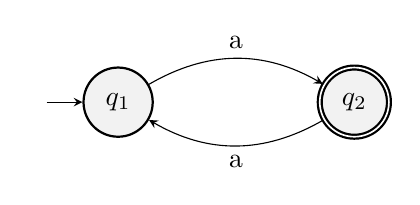
\begin{tikzpicture}
\node[state, initial] (q1) {$q_1$};
\node[state, accepting, right of=q1] (q2) {$q_2$};
\draw
(q1) edge[bend left, above] node{a} (q2)
(q2) edge[bend left, below] node{a} (q1);
\end{tikzpicture}
\\
Da un primo sguardo al diagramma possiamo notare che la parola "\mbox{$a$}" viene accettata da \mbox{$A_1$}.
Invece la parola "\mbox{$aa$}" non è altrettanto fortunata. Altre parole accettate sono "\mbox{$aaa$}",
"\mbox{$aaaaa$}", "\mbox{$aaaaaaa$}".
Altre parole non accettate sono: \mbox{$\epsilon$}, "\mbox{$aaaa$}", "\mbox{$aaaaaa$}". Sembra che questo automa
accetti soltanto le parole di lunghezza dispari.



\subsubsection{Linguaggio di un DFA}

Dato un DFA \mbox{$A = (Q, \Sigma, \delta, q_0, F)$}, si definisce il linguaggio riconosciuto da \mbox{$A$}:
\\

\mbox{$L(A) = \{ w | A \text{ accetta } w \}$}
\\
\\
Per esprimere in modo più formale "\mbox{$A \text{ accetta } w$}" si introduce il concetto di
\textit{funzione di transizione estesa} \mbox{$\hat\delta \colon Q \times \Sigma^* \to Q$}.
\\
\\
Passo base
\\
\mbox{$\hat\delta(q, \epsilon) = q, \forall q \in Q$}
\\
\\
Passo ricorsivo \mbox{$\forall q \in Q, w \in \Sigma^*, a \in \Sigma$}
\\
\mbox{$\hat\delta(q, wa) = \delta(\hat\delta(q, w), a)$}
\\
\\
La \textit{funzione di transizione estesa} \mbox{$\hat\delta$} (chiamata "\textit{delta cappello}") fornisce
lo stato finale del relativo DFA alla fine della computazione dati stringa in input e stato di partenza.
Se viene usata per seguire una computazione di un automa a partire dal suo stato iniziale e una parola in
input, e si ottiene come risultato uno stato finale, allora la parola in input è accettata da tale automa.
\\
\\
Quindi è possibile riscrivere la definizione di linguaggio riconosciuto come segue.
\\
\mbox{$L(A) = \{ w | \hat\delta(q_0, w) \in F \}$}.



\subsubsection{Esempio di applicazione di funzione di transizione estesa}

Prendendo in considerazione l'automa \mbox{$A_1$} in \textbf{3.1.1} è possibile verificare quanto segue.
\\
\\
\mbox{$ \hat\delta(q_1, \epsilon) = q_1 \not\in F $}
\\
\mbox{$ \hat\delta(q_1, a) = \delta( \hat\delta(q_1, \epsilon) , a) = \delta( q_1 , a) = q_2 \in F $}
\\
\mbox{$ \hat\delta(q_1, aa) = \delta( \hat\delta(q_1, a) , a) = \delta( q_2 , a) = q_1 \not\in F $}
\\
\mbox{$ \hat\delta(q_1, aaa) = \delta( \hat\delta(q_1, aa) , a) = \delta( q_1 , a) = q_2 \in F $}
\\
\mbox{$ \hat\delta(q_1, aaaa) = \delta( \hat\delta(q_1, aaa) , a) = \delta( q_2 , a) = q_1 \not\in F $}
\\
\mbox{$ \hat\delta(q_1, aaaaa) = \delta( \hat\delta(q_1, aaaa) , a) = \delta( q_1 , a) = q_2 \in F $}
\\
\mbox{$ \hat\delta(q_1, aaaaaa) = \delta( \hat\delta(q_1, aaaaa) , a) = \delta( q_2 , a) = q_1 \not\in F $}
\\
\mbox{$ \hat\delta(q_1, aaaaaaa) = \delta( \hat\delta(q_1, aaaaaa) , a) = \delta( q_1 , a) = q_2 \in F $}



\subsubsection{Estensione di una funzione}

Siano \mbox{$f \colon B \to T, g \colon A \to T$} due funzioni con \mbox{$ B \subseteq A $}.
\\
\mbox{$ g \text{ estensione di } f \overset{\text{def}}{\Leftrightarrow} g(x) = f(x), \forall x \in B $}
\\
\\
Allo stesso modo, sia \mbox{$h \colon C \to T$} una funzione con \mbox{$ C \subseteq B $}.
\\
\mbox{$ h \text{ riduzione di } f \overset{\text{def}}{\Leftrightarrow} h(x) = f(x), \forall x \in C $}
\\
\\
Banalmente, la funzione di transizione estesa \mbox{$ \hat\delta $} è una estensione della funzione di
transizione \mbox{$ \delta $} dato che \mbox{$ \Sigma \subseteq \Sigma^* $}
(quindi \mbox{$ (Q \times \Sigma) \subseteq (Q \times \Sigma^*) $}) e:
\\
\mbox{$ \forall (q, a) \in Q \times \Sigma $}
\\
\mbox{$ \hat\delta(q, a) = \delta(\hat\delta(q, \epsilon), a) = \delta(q, a) $}



\subsubsection{Altri esempi di DFA}

Si considerino i seguenti automi, rispettivamente \mbox{$A_1$} e \mbox{$A_2$}.
\\
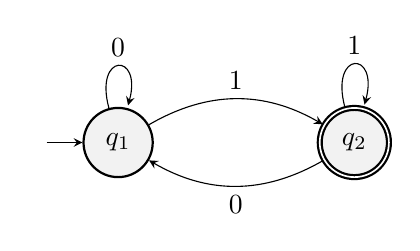
\begin{tikzpicture}
\node[state, initial] (q1) {$q_1$};
\node[state, accepting, right of=q1] (q2) {$q_2$};
\draw
(q1) edge[loop above]       node{0} (q1)
(q1) edge[bend left, above] node{1} (q2)
(q2) edge[loop above]       node{1} (q2)
(q2) edge[bend left, below] node{0} (q1);
\end{tikzpicture}
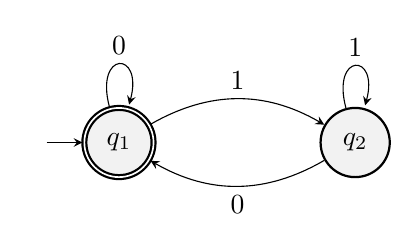
\begin{tikzpicture}
\node[state, initial, accepting] (q1) {$q_1$};
\node[state, right of=q1] (q2) {$q_2$};
\draw
(q1) edge[loop above]       node{0} (q1)
(q1) edge[bend left, above] node{1} (q2)
(q2) edge[loop above]       node{1} (q2)
(q2) edge[bend left, below] node{0} (q1);
\end{tikzpicture}
\\
\\
Dopo una osservazione, è possibile riconscere che \mbox{$ L(A_1) = \{ w1 | w \in \{ 0, 1 \}* \} $}.
Inoltre, il linguaggio riconosciuto da \mbox{$A_2$} sembra accettare tutte le parole possibili tranne
quelle accettate da \mbox{$A_1$}.
\\
Infatti, \mbox{$ L(A_2) = \{ 0, 1 \}^* / \{ w1 | w \in \{ 0, 1 \}* \} = \{ 0, 1 \}^* / L(A_1) $} è il
complemento del linguaggio \mbox{$L(A_1)$}.
\\
Si noti che l'unica differenza nella definizioni di \mbox{$A_1$} e \mbox{$A_2$} è che i rispettivi
insiemi di stati finali sono tra loro complementari. In seguito saranno forniti maggiori dettagli sulla
relazione tra un DFA e il suo DFA complementare.


\newpage
Si consideri il seguente automa \mbox{$A_3$}.
\\
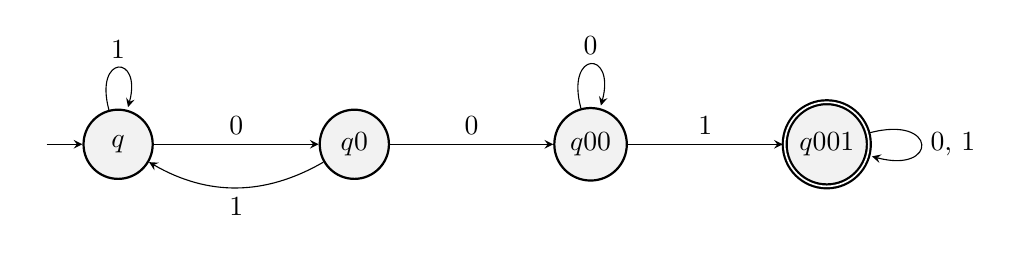
\begin{tikzpicture}
\node[state, initial]                 (q)    {$q$};
\node[state, right of=q]              (q0)   {$q0$};
\node[state, right of=q0]             (q00)  {$q00$};
\node[state, accepting, right of=q00] (q001) {$q001$};
\draw
(q)    edge[loop above]       node{1} (q)
(q)    edge[above]            node{0} (q0)
(q0)   edge[above]            node{0} (q00)
(q0)   edge[bend left, below] node{1} (q)
(q00)  edge[above]            node{1} (q001)
(q00)  edge[loop above]       node{0} (q0)
(q001) edge[loop right]       node{0, 1} (q001);
\end{tikzpicture}
\\
\\
\mbox{$L(A_3) = \{ x001y | x, y \in \{ 0, 1 \}* \}$}
\\
\\
\\
Si consideri il seguente automa \mbox{$A_4$}.
\\
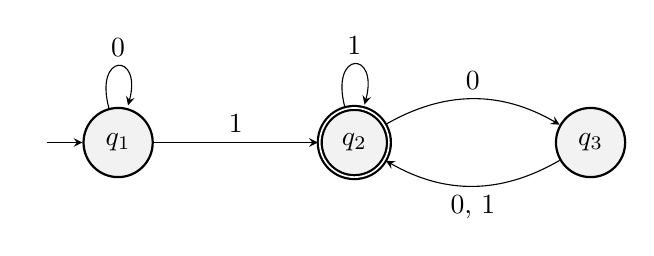
\begin{tikzpicture}
\node[state, initial]                (q1) {$q_1$};
\node[state, accepting, right of=q1] (q2) {$q_2$};
\node[state, right of=q2]            (q3) {$q_3$};
\draw
(q1)   edge[loop above]       node{0} (q1)
(q1)   edge[above]            node{1} (q2)
(q2)   edge[loop above]       node{1} (q2)
(q2)   edge[bend left, above]            node{0} (q3)
(q3)   edge[bend left, below]            node{0, 1} (q2);
\end{tikzpicture}
\\
\\
\mbox{$ L(A_4) = L( 0^* 1 ( 1 + 0 \Sigma )^* )
= \text{ ... }
= \{ w1(00)^{2k} | w \in \Sigma^*, k \in \mathbf{N_0} \}$}
\\
\\
\\
Si consideri il seguente automa \mbox{$A_5$}.
\\
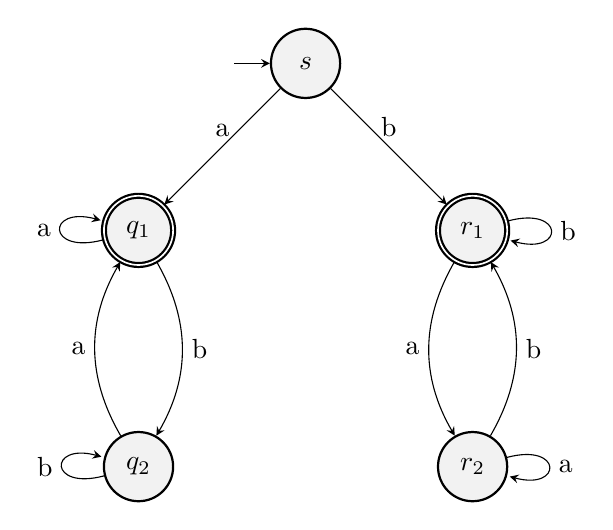
\begin{tikzpicture}
\node[state, initial]                     (s)  {$s$};
\node[state, accepting, below left of=s]  (q1) {$q_1$};
\node[state, below of=q1]      (q2) {$q_2$};
\node[state, accepting, below right of=s] (r1) {$r_1$};
\node[state, below of=r1]      (r2) {$r_2$};
\draw
(s)   edge[above] node{a} (q1)
(s)   edge[above] node{b} (r1)
(q1)   edge[loop left]        node{a} (q1)
(q1)   edge[bend left, right] node{b} (q2)
(q2)   edge[loop left]        node{b} (q2)
(q2)   edge[bend left, left]  node{a} (q1)
(r1)   edge[loop right]        node{b} (r1)
(r1)   edge[bend right, left]  node{a} (r2)
(r2)   edge[loop right]        node{a} (r2)
(r2)   edge[bend right, right] node{b} (r1);
\end{tikzpicture}
\\
\\
\mbox{$ L(A_5) =
\{ w | w \text{ inizia e termina con lo stesso carattere su } \{ a, b \} \}$}



\newpage
Si intende dimostrare che
\mbox{$ L(A_p) = \{ a^n | n \text{ pari} \} $}. Ecco una
rappresentazione grafica dell'automa \mbox{$A_p$}.
\\
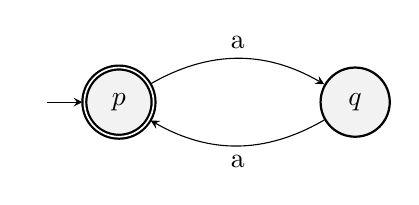
\begin{tikzpicture}
\node[state, initial, accepting] (p) {$p$};
\node[state, right of=p] (q) {$q$};
\draw
(p) edge[bend left, above] node{a} (q)
(q) edge[bend left, below] node{a} (p);
\end{tikzpicture}
\\
Sarà usato il principio di induzione per dimostrare la proposizione
\\
\mbox{$ P(n) \colon a^n \in L(A_p) \Leftrightarrow n \text{ pari} $}.
\\
\\
Passo base: \mbox{$ 0 \text{ pari}, a^0 = \epsilon \in L(A_p)
\text{ dato che }
\hat\delta(p, \epsilon) = p$}
\\
\\
Passo induttivo: dimostrare \mbox{$ P(n) \Rightarrow P(n + 1) $}.
\\
\\
Dimostrazione 1: \mbox{$ a^{n + 1} \in L(A_p) \Rightarrow n + 1 \text{ pari} $}.
\\
\begin{math}
a^{n + 1} \in L(A_p)
\Rightarrow \hat\delta(p, a^{n + 1}) = p \in F_{A_p}
\Rightarrow \hat\delta(p, a^n) = q \not\in F_{A_p}
\Rightarrow a^n \not\in L(A_p) \\
\Rightarrow \text{ (per ipotesi induttiva) } n \text{ dispari}
\Rightarrow n + 1 \text{ pari}
\end{math}
\\
\\
Dimostrazione 2: \mbox{$ n + 1 \text{ pari} \Rightarrow a^{n + 1} \in L(A_p) $}.
\\
\begin{math}
n + 1 \text{ pari}
\Rightarrow n \text{ dispari} \\
\Rightarrow \text{ (per ipotesi induttiva) } a^n \not\in L(A_p)
\Rightarrow \hat\delta(p, a^n) = q \\
\Rightarrow \hat\delta(p, a^{n + 1}) = \delta(\hat\delta(p, a^n), a) = \delta(q, a) = p \in F_{A_p}
\Rightarrow a^{n + 1} \in L(A_p)
\end{math}
\\
\\
Per dimostrare solo una direzione di \mbox{$ P(n) $} suggerisco di usare
l'induzione forte.


\newpage
\subsubsection{Linguaggi regolari}

Sia \mbox{$ L $} linguaggio su \mbox{$ \Sigma $}.
\\
\\
\mbox{$ L \text{ regolare }
\overset{\text{def}}{\Leftrightarrow}
\exists \text{ DFA } A \colon L(A) = L $}
\\
\\
La classe dei linguaggi regolari è chiamata \mbox{$ REG $}.



\subsubsection{Chiusura classe rispetto a una operazione}

Una classe di oggetti è chiusa rispetto a una operazione se l'applicazione di questa operazione su
elementi appartenenti alla classe restituisce un oggetto anch'esso appartenente alla classe.
\\
\\
Come vedremo, la classe \mbox{$ REG $} è chiusa rispetto alle operazioni complemento, unione
e intersezione.



\subsubsection{Chiusura dei linguaggi regolari rispetto al complemento}

La classe \mbox{$ REG $} è chiusa rispetto all'operazione complemento. Sia \mbox{$ L \in REG $} e
\mbox{$ L = L(A) $} con \mbox{$ A $} DFA. Allora
\mbox{$ \exists \bar{A} \text{ DFA} \colon L(\bar{A}) = \bar{L} $}.
\\
\\
Dimostrazione:
\\
...



\subsubsection{Chiusura dei linguaggi regolari rispetto a unione e intersezione}

...



\section*{Conclusioni}

...



\end{document}
